\documentclass[aspectratio=169]{../latex_main/tntbeamer}  % you can pass all options of the beamer class, e.g., 'handout' or 'aspectratio=43'
\usepackage{dsfont}
\usepackage{bm}
\usepackage[english]{babel}
\usepackage[T1]{fontenc}
%\usepackage[utf8]{inputenc}
\usepackage{graphicx}
\graphicspath{ {./figures/} }
\usepackage{algorithm}
\usepackage[ruled,vlined,algo2e,linesnumbered]{algorithm2e}
\usepackage{hyperref}
\usepackage{booktabs}
\usepackage{mathtools}

\usepackage{amsmath,amssymb}

\DeclareMathOperator*{\argmax}{arg\,max}
\DeclareMathOperator*{\argmin}{arg\,min}

\usepackage{amsbsy}
\newcommand{\vect}[1]{\bm{#1}}
%\newcommand{\vect}[1]{\boldsymbol{#1}}

\usepackage{pgfplots}
\pgfplotsset{compat=1.16}
\usepackage{tikz}
\usetikzlibrary{trees} 
\usetikzlibrary{shapes.geometric}
\usetikzlibrary{positioning,shapes,shadows,arrows,calc,mindmap}
\usetikzlibrary{positioning,fadings,through}
\usetikzlibrary{decorations.pathreplacing}
\usetikzlibrary{intersections}
\pgfdeclarelayer{background}
\pgfdeclarelayer{foreground}
\pgfsetlayers{background,main,foreground}
\tikzstyle{activity}=[rectangle, draw=black, rounded corners, text centered, text width=8em]
\tikzstyle{data}=[rectangle, draw=black, text centered, text width=8em]
\tikzstyle{myarrow}=[->, thick, draw=black]

% Define the layers to draw the diagram
\pgfdeclarelayer{background}
\pgfdeclarelayer{foreground}
\pgfsetlayers{background,main,foreground}

% Requires XeLaTeX or LuaLaTeX
%\usepackage{unicode-math}

\usepackage{fontspec}
%\setsansfont{Arial}
\setsansfont{RotisSansSerifStd}[ 
Path=../latex_main/fonts/,
Extension = .otf,
UprightFont = *-Regular,  % or *-Light
BoldFont = *-ExtraBold,  % or *-Bold
ItalicFont = *-Italic
]
\setmonofont{Cascadia Mono}[
Scale=0.8
]

% scale factor adapted; mathrm font added (Benjamin Spitschan @TNT, 2021-06-01)
%\setmathfont[Scale=1.05]{Libertinus Math}
%\setmathrm[Scale=1.05]{Libertinus Math}

% other available math fonts are (not exhaustive)
% Latin Modern Math
% XITS Math
% Libertinus Math
% Asana Math
% Fira Math
% TeX Gyre Pagella Math
% TeX Gyre Bonum Math
% TeX Gyre Schola Math
% TeX Gyre Termes Math

% Literature References
\newcommand{\lit}[2]{\href{#2}{\footnotesize\color{black!60}[#1]}}

%%% Beamer Customization
%----------------------------------------------------------------------
% (Don't) Show sections in frame header. Options: 'sections', 'sections light', empty
\setbeamertemplate{headline}{empty}

% Add header logo for normal frames
\setheaderimage{
	% 
\includegraphics[height=\logoheight]{figures/TNT_darkv4.pdf}
	
\includegraphics[height=\logoheight]{../latex_main/figures/luh_logo_rgb_0_80_155.pdf}
	% 
\includegraphics[height=\logoheight]{figures/logo_tntluh.pdf}
}

% Header logo for title page
\settitleheaderimage{
	% 
\includegraphics[height=\logoheight]{figures/TNT_darkv4.pdf}
	
\includegraphics[height=\logoheight]{../latex_main/figures/luh_logo_rgb_0_80_155.pdf}
	% 
\includegraphics[height=\logoheight]{figures/logo_tntluh.pdf}
}

% Title page: tntdefault 
\setbeamertemplate{title page}[tntdefault]  % or luhstyle
% Add optional title image here
%\addtitlepageimagedefault{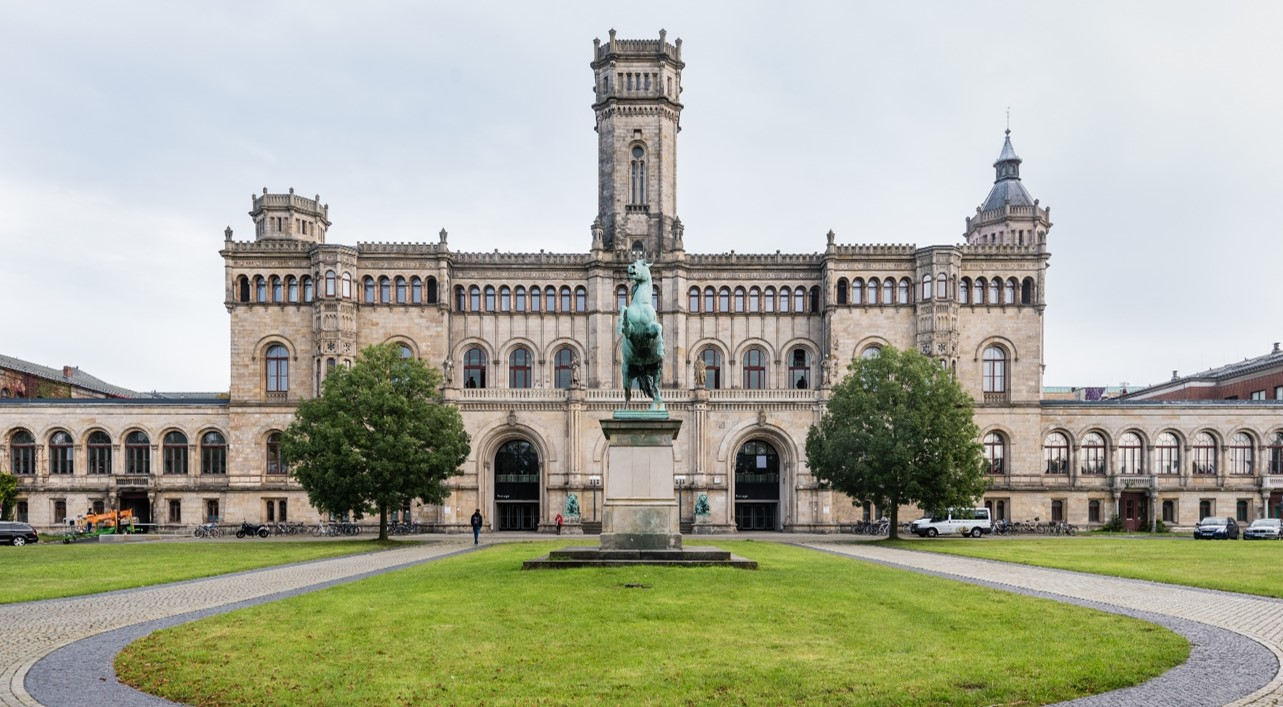
\includegraphics[width=0.65\textwidth]{figures/luh_default_presentation_title_image.jpg}}

% Title page: luhstyle
% \setbeamertemplate{title page}[luhstyle]
% % Add optional title image here
% \addtitlepageimage{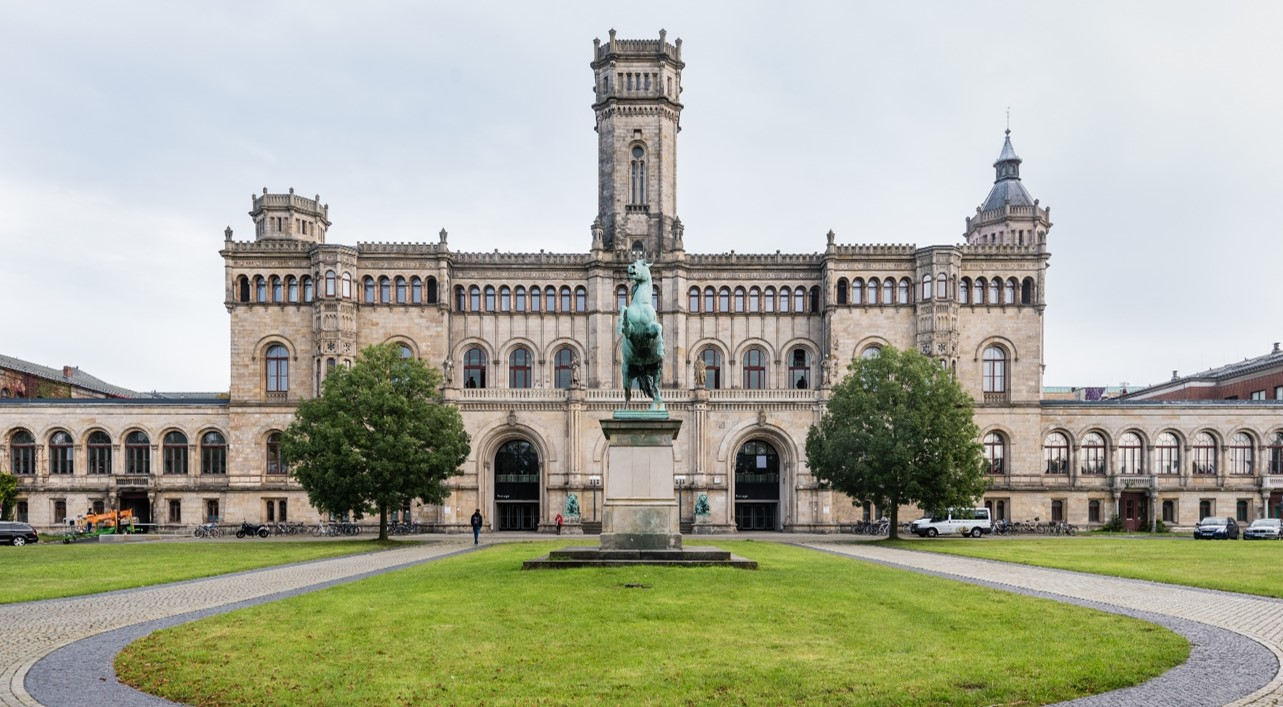
\includegraphics[width=0.75\textwidth]{figures/luh_default_presentation_title_image.jpg}}

\author[Abedjan \& Lindauer]{Ziawasch Abedjan \& Marius Lindauer\\[1em]
	
\includegraphics[height=\logoheight]{../latex_main/figures/luh_logo_rgb_0_80_155.pdf}\qquad
	
\includegraphics[height=\logoheight]{../latex_main/figures/DBIS_Kurzlogo.png}\qquad

\includegraphics[height=\logoheight]{../latex_main/figures/TNT_darkv4}\qquad

\includegraphics[height=\logoheight]{../latex_main/figures/L3S.jpg}	}
\date{Summer Term 2022; \hspace{0.5em} {
\includegraphics[height=1.5em]{../latex_main/figures/Cc-by-nc-sa_icon.svg.png}}; based on \href{https://ds100.org/fa21/}{[DS100]}
}


%%% Custom Packages
%----------------------------------------------------------------------
% Create dummy content
\usepackage{blindtext}

% Adds a frame with the current page layout. Just call \layout inside of a frame.
\usepackage{layout}


%%% Macros
%\renewcommand{\vec}[1]{\mathbf{#1}}
% \usepackage{bm}
%\let\vecb\bm

\title[Introduction]{DS: Logistic Regression, Classification}
\subtitle{Evaluating classifiers}

\graphicspath{ {./figure/} }
%\institute{}


\begin{document}
	
	\maketitle
	\begin{frame}{Accuracy}
	    \begin{itemize}
	        \item Now that we actually have our classifier, let’s try and quantify how well it performs.
	        \item The most basic evaluation metric for a classifier is accuracy.
	        \begin{itemize}
	            \item Widely used.
	            \item model.score in scikit-learn calculates this.
	            \item Changing the threshold can change our model’s accuracy (will explore soon).
	            \item In the presence of class imbalance – not so meaningful!
	        \end{itemize}
	    \end{itemize}
	    \begin{equation*}
	        \text{accuracy} = \frac{\# \text{of points classified correctly}}{\# \text{points total}}
	    \end{equation*}
	\end{frame}
	
	
	\begin{frame}[c]{Pitfalls of accuracy}
	    \begin{columns}
	        \begin{column}{.5\textwidth}
                 Suppose we’re trying to build a classifier to filter spam emails.
        	    \begin{itemize}
        	        \item Each email is spam (1) or ham (0).
        	    \end{itemize}
        	    Let’s say we have 100 emails, of which 5 are truly spam, and the remaining 95 are ham.
        	    \begin{itemize}
        	        \item Your friend suggests you classify every email as ham.
        	        \item What is the accuracy of your friend’s classifier?
        	        \item Is accuracy a good metric of this classifier’s performance?
        	    \end{itemize}
	        \end{column}
	        
	        
	        \begin{column}{.5\textwidth}
	                
	        \end{column}
	    \end{columns}
	   
	\end{frame}
	
	
	
	\begin{frame}[c]{Pitfalls of accuracy}
	    \begin{columns}
	        \begin{column}{.5\textwidth}
                 Suppose we’re trying to build a classifier to filter spam emails.
        	    \begin{itemize}
        	        \item Each email is spam (1) or ham (0).
        	    \end{itemize}
        	    Let’s say we have 100 emails, of which 5 are truly spam, and the remaining 95 are ham.
        	    \begin{itemize}
        	        \item Your friend suggests you classify every email as ham.
        	        \item What is the accuracy of your friend’s classifier?
        	        \item Is accuracy a good metric of this classifier’s performance?
        	    \end{itemize}
	        \end{column}
	        
	        
	        \begin{column}{.5\textwidth}
	                Accuracy is 95\%.
                    \begin{itemize}
                        \item But we didn’t detect any spam emails!
                        \item Alternative: classify everything as spam.
                        \begin{itemize}
                            \item We’d catch all spam emails!
                            \item But we’d also have a bunch of non-spam emails classified as spam.
                        \end{itemize}
                        \item This suggests we need to be looking at more than just accuracy.
                    \end{itemize}
	        \end{column}
	    \end{columns}
	   
	\end{frame}
	
	
	
	\begin{frame}[c]{Types of classification errors}
	    \begin{columns}
	        \begin{column}{.5\textwidth}
                 Moving forward, “positive” refers to 1 and “negative” refers to 0.
        	    \begin{itemize}
        	        \item True positives and true negatives are when we correctly classify an observation as being positive or negative.
        	        \item False positives are like “false alarms.”
        	        \item False negatives are when we “fail to detect” things.
        	    \end{itemize}
	        \end{column}
	        
	        
	        \begin{column}{.5\textwidth}
	                \begin{figure}
	                    \centering
	                    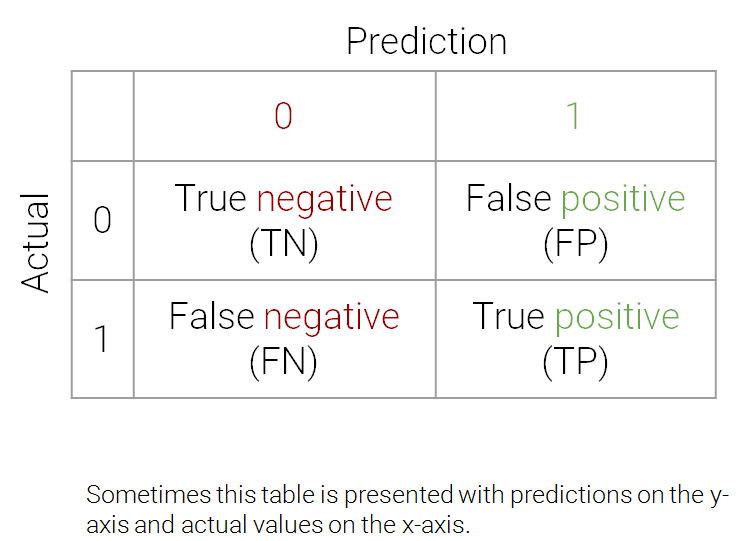
\includegraphics[scale=.38]{Bild7}
	                \end{figure}
	        \end{column}
	    \end{columns}
	   
	\end{frame}
	
	
	\begin{frame}{Confusion matrix}
	    A confusion matrix gives us the four quantities on the previous slide, for a particular classifier and set of data.
	    \begin{figure}
	        \centering
	        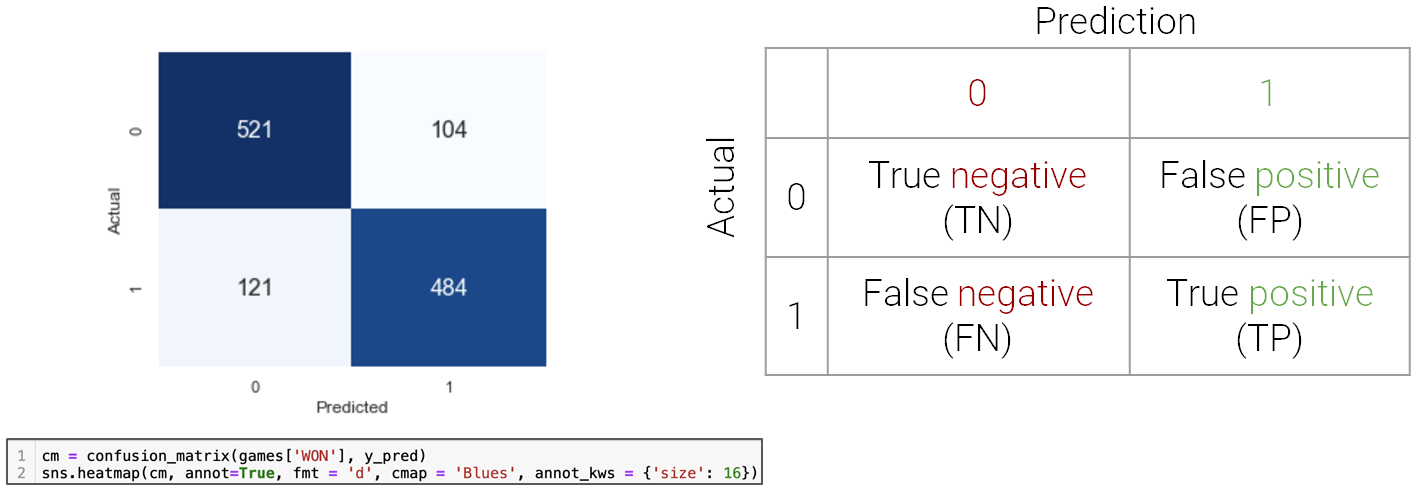
\includegraphics[scale=.4]{Bild8}
	    \end{figure}
	\end{frame}
	
	
	\begin{frame}{Precision and recall}
	  \begin{columns}
	      \begin{column}{.5\textwidth}
	              \begin{align*}
	                  \text{accuracy} = \frac{TP + TN}{n}
	                  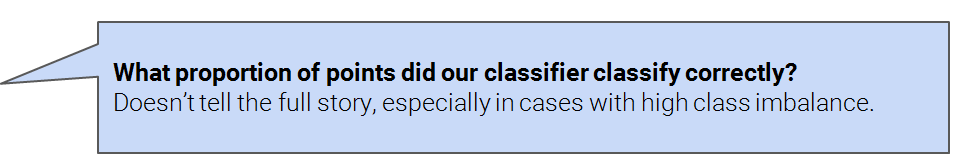
\includegraphics[scale=.35]{Bild9}\\
	                  \text{precision} = \frac{TP}{TP + FP}
	                  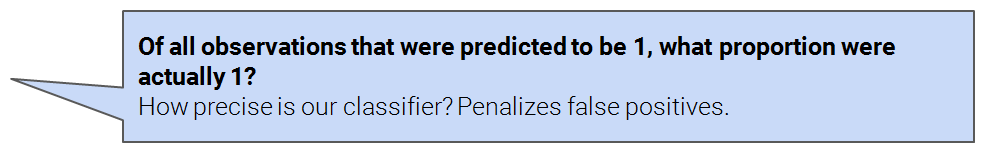
\includegraphics[scale=.35]{Bild10}\\
	                  \text{recall} = \frac{TP}{TP + FN}
	                  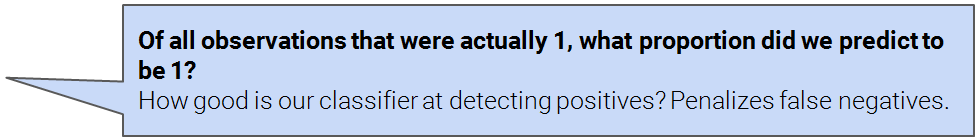
\includegraphics[scale=.35]{Bild11}
	              \end{align*}
	      \end{column}
	      
	      
	      \begin{column}{.2\textwidth}
	             \begin{figure}
	                 \centering
	                 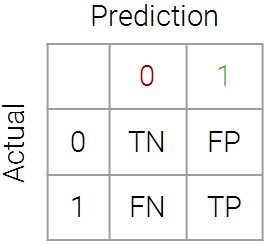
\includegraphics[scale=.4]{Bild12}
	             \end{figure} 
	      \end{column}
	  \end{columns}
	\end{frame}
	
	
	
	\begin{frame}{Precision and recall}
	  \begin{columns}
	      \begin{column}{.5\textwidth}
	              \begin{align*}
	                  \text{accuracy} = \frac{TP + TN}{n}
	                  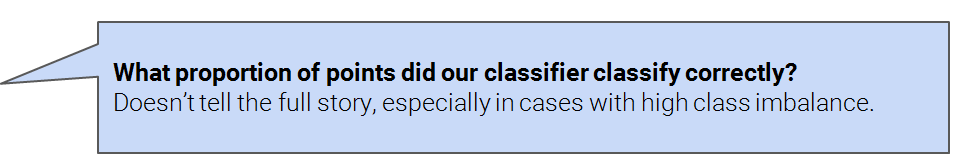
\includegraphics[scale=.35]{Bild9}\\
	                  \text{precision} = \frac{TP}{TP + FP}
	                  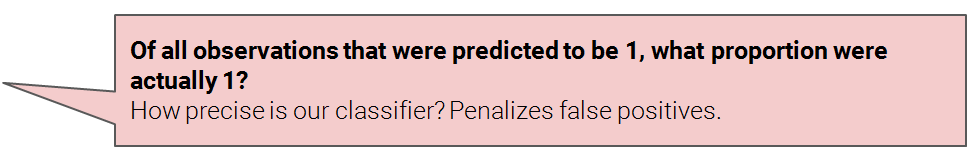
\includegraphics[scale=.35]{Bild13}\\
	                  \text{recall} = \frac{TP}{TP + FN}
	                  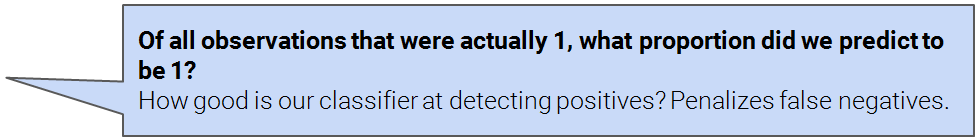
\includegraphics[scale=.35]{Bild11}
	              \end{align*}
	      \end{column}
	      
	      
	      \begin{column}{.2\textwidth}
	             \begin{figure}
	                 \centering
	                 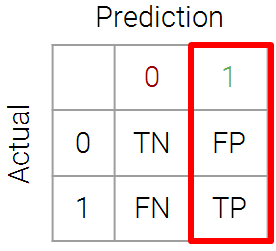
\includegraphics[scale=.4]{Bild14}
	             \end{figure} 
	      \end{column}
	  \end{columns}
	\end{frame}
	
	
	
	\begin{frame}{Precision and recall}
	  \begin{columns}
	      \begin{column}{.5\textwidth}
	              \begin{align*}
	                  \text{accuracy} = \frac{TP + TN}{n}
	                  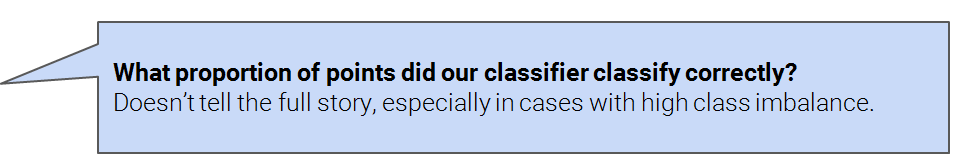
\includegraphics[scale=.35]{Bild9}\\
	                  \text{precision} = \frac{TP}{TP + FP}
	                  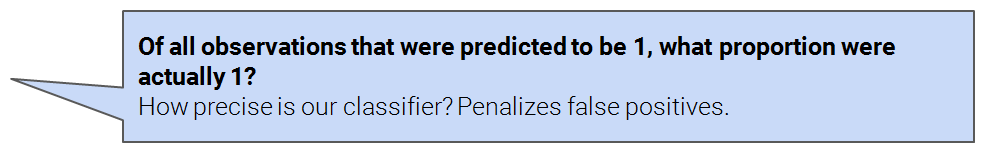
\includegraphics[scale=.35]{Bild10}\\
	                  \text{recall} = \frac{TP}{TP + FN}
	                  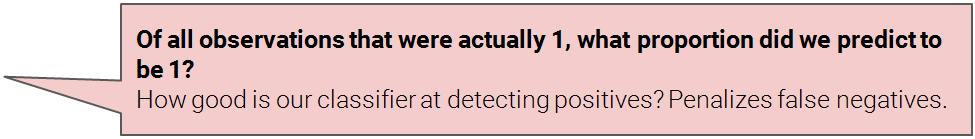
\includegraphics[scale=.35]{Bild15}
	              \end{align*}
	      \end{column}
	      
	      
	      \begin{column}{.2\textwidth}
	             \begin{figure}
	                 \centering
	                 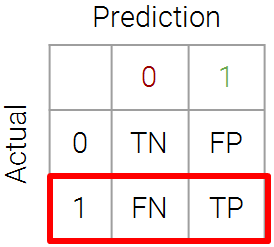
\includegraphics[scale=.4]{Bild16}
	             \end{figure} 
	      \end{column}
	  \end{columns}
	\end{frame}
	
	
	
	\begin{frame}{Precision and recall}
	  \begin{columns}
	        \begin{column}{.5\textwidth}
                 Suppose we’re trying to build a classifier to filter spam emails.
        	    \begin{itemize}
        	        \item Each email is spam (1) or ham (0).
        	    \end{itemize}
        	    Let’s say we have 100 emails, of which 5 are truly spam, and the remaining 95 are ham.
        	    \begin{itemize}
        	        \item Your friend suggests you classify every email as ham.
        	        \item What is the accuracy?
        	        \item What is the precision?
        	        \item What is the recall?
        	    \end{itemize}
	        \end{column}
	        
	        
	        \begin{column}{.5\textwidth}
	                Accuracy is 95\%.
                    \begin{itemize}
                        \item But we didn’t detect any spam emails!
                        \item Alternative: classify everything as spam.
                        \begin{itemize}
                            \item We’d catch all spam emails!
                            \item But we’d also have a bunch of non-spam emails classified as spam.
                        \end{itemize}
                        \item This suggests we need to be looking at more than just accuracy.
                    \end{itemize}
	        \end{column}
	    \end{columns}
	\end{frame}
	
	
	
	\begin{frame}{Precision and recall}
	  \begin{columns}
	        \begin{column}{.5\textwidth}
                 Suppose we’re trying to build a classifier to filter spam emails.
        	    \begin{itemize}
        	        \item Each email is spam (1) or ham (0).
        	    \end{itemize}
        	    Let’s say we have 100 emails, of which 5 are truly spam, and the remaining 95 are ham.
        	    \begin{itemize}
        	        \item Your friend suggests you classify every email as ham.
        	        \item What is the accuracy?
        	        \item What is the precision?
        	        \item What is the recall?
        	    \end{itemize}
	        \end{column}
	        
	        
	        \begin{column}{.5\textwidth}
	               TP = 0, FP = 0, TN = 95, FN = 5\\
	               \bigskip
	               Accuracy = 95\%\\
	               Precision = 0 / (0 + 0) = undefined\\
	               Recall = 0 / (0 + 5) = 0\%\\
	               \bigskip
	               Accuracy doesn’t tell the full story.
                    \begin{itemize}
                        \item Class imbalance – the distribution of true observations is skewed
                        \item Here, 95\% of true observations are negative.
                    \end{itemize}
	        \end{column}
	    \end{columns}
	\end{frame}
	
	
	\begin{frame}{Trade-off between precision and recal}
	    \begin{columns}
	      \begin{column}{.8\textwidth}
	              \begin{itemize}
	                  \item Precision penalizes false positives, and recall penalizes false negatives.
	                  \item We can achieve 100\% recall by making our classifier output “1”, regardless of the input.
	                  \begin{itemize}
	                      \item We would have no false negatives, but many false positives, and so our precision would be low.
	                  \end{itemize}
	                  \item This suggests that there is a tradeoff between precision and recall – they are inversely related. 
	                  \begin{itemize}
	                      \item Ideally, both would be near 100\%, but that’s unlikely to happen.
	                  \end{itemize}
	                  \item We can adjust our classification threshold to suit our needs, depending on the domain.
	                  \begin{itemize}
	                      \item Higher threshold – fewer false positives. Precision tends to increase.
	                      \item Lower threshold – fewer false negatives. Recall increases.
	                  \end{itemize}
	              \end{itemize}
	      \end{column}
	      
	      
	      \begin{column}{.2\textwidth}
	             \begin{figure}
	                 \centering
	                 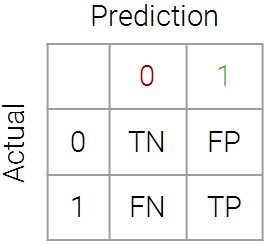
\includegraphics[scale=.4]{Bild12}
	             \end{figure} 
	      \end{column}
	  \end{columns}
	\end{frame}
	
	\begin{frame}{Examples}
	    In each of the following cases, what would we want to maximize: precision, recall, or accuracy?\\
	    \begin{itemize}
	        \item Predicting whether or not a patient has some disease.
	        \item Determining whether or not someone should be sentenced to life in prison.
	        \item  Determining if an email is spam or ham.
	    \end{itemize}
	\end{frame}
	
	
	\begin{frame}{Examples}
	    In each of the following cases, what would we want to maximize: precision, recall, or accuracy?\\
	    \begin{itemize}
	        \item Predicting whether or not a patient has some disease.
	        \begin{itemize}
	            \item Maximize recall.
	            \item Presumably if we say someone has the disease, they will go through further testing.
	            \item If we say they don’t, the condition may be left untreated, which is dangerous.
	        \end{itemize}
	        \item Determining whether or not someone should be sentenced to life in prison.
	        \begin{itemize}
	            \item Maximize precision.
	            \item We don’t want to sentence innocent people, so we want to be very sure that this is a true positive.
	        \end{itemize}
	        \item  Determining if an email is spam or ham.
	        \begin{itemize}
	            \item Maximize accuracy, though this one is subjective.
	            \item Depends what you think is worse – having a bunch of spam emails ending up in your inbox, or a bunch of non-spam emails being filtered out. 
	        \end{itemize}
	    \end{itemize}
	\end{frame}
\end{document}